
\subsection{Design Elements}
\label{sec:design-elements}

%-------------------------------------------------------------%
\subsubsection{Hardware Elements}
\temp{To-add}

%-------------------------------------------------------------%
\subsubsection{Firmware Elements}

The firmware elements, which are described in Fig.~\ref{fig:block-software}, are described in detail below. The detailed implementation of these elements in given in \cite{flightcontroller_git}.

%-------------------------------%
\paragraph{\textbf{Sensor Task} \textit{sensors.c}} \leavevmode

The sensor task provides an interface for the \gls{mpu6050} 6-axis \gls{imu} through \gls{i2c}, which provides real-time data from the accelerometer and gyroscope on the sensor. This is done on a register level using Espressif's \textit{I2C} library.

The raw data obtained from the \gls{mpu6050} sensor are 16-bit integer values representing the gyroscope and accelerometer measurements. These values are first converted into physical units (SI units) based on the selected sensitivity configuration of the sensor. The conversion from raw readings to angular velocity and linear acceleration is expressed as:

\begin{align}
\boldsymbol{\omega} &= (\mathbf{G}_{\text{raw}} - \mathbf{G}_{\text{bias}}) \times S_{\text{gyro}}, \\[6pt]
\mathbf{a} &= \mathbf{A}_{\text{raw}} \times S_{\text{acc}},
\end{align}

where \( \mathbf{G}_{\text{raw}} \) and \( \mathbf{A}_{\text{raw}} \) are the raw gyroscope and accelerometer readings, 
\( \mathbf{G}_{\text{bias}} \) is the gyroscope bias, which is calculated when the filter is intialised. \( S_{\text{gyro}} \) and \( S_{\text{acc}} \) are the corresponding sensitivity scaling factors.

To reduce measurement noise, a second-order digital biquad low-pass filter is applied to the sensor data. This filter attenuates high-frequency noise while preserving the motion dynamics of interest. Cutoff frequencies of 30\,Hz and 80\,Hz are used for the accelerometer and gyroscope, respectively. Additionally, the \gls{mpu6050} incorporates an internal digital low-pass filter on the gyroscope measurements, which is also enabled for further signal smoothing.

The digital biquad filter can be expressed in the $z$-domain as:

\begin{align}
H(z) &= \frac{b_0 + b_1 z^{-1} + b_2 z^{-2}}{1 + a_1 z^{-1} + a_2 z^{-2}}, \\[6pt]
w(n) &= x(n) - a_1 w(n-1) - a_2 w(n-2), \\[6pt]
y(n) &= b_0 w(n) + b_1 w(n-1) + b_2 w(n-2),
\end{align}

where \( x(n) \) is the current input sample, \( y(n) \) is the filtered output, and \( w(n) \) represents the internal state variables in Direct Form~II. The coefficents can be found in \textit{filter.c}.

A interrupt service routine (ISR) is attached to the \gls{mpu6050} interrupt, this means that instead of the sensor task continuously reading from the \gls{mpu6050}, it waits for the trigger to signify that data is ready to be read. The data is then stored for a queue and an additional signal is sent for the stabiliser task to signify the processed sensor data is ready.

\begin{figure}[H]
    \centering
    \captionsetup{justification=centering, margin=1cm}
    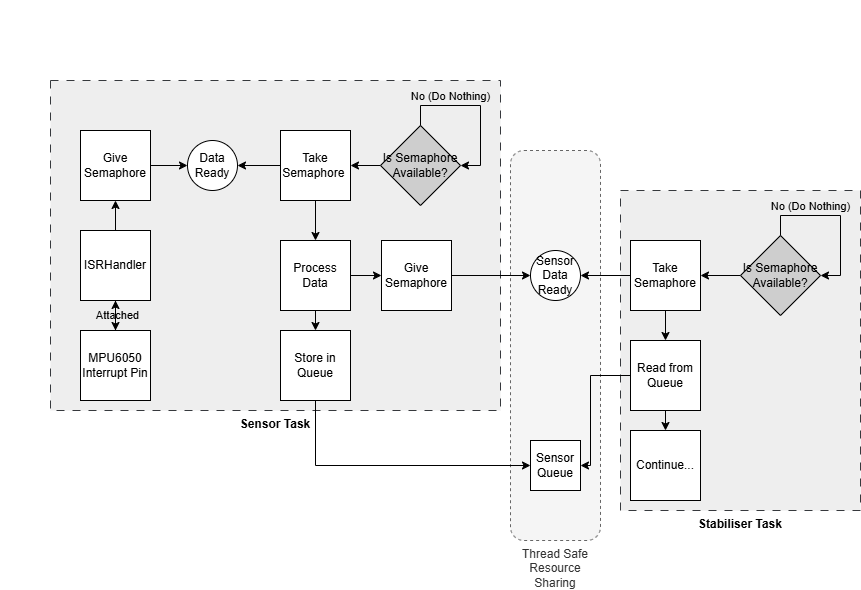
\includegraphics[width=0.9\textwidth]{img/sensor-semaphore.PNG}
    \caption{Thread-safe Data Availability Signalling Heurisitic}
    \label{fig:arch-process}
\end{figure}

The code for this can be found in \ref{app:sensor-code}.

%-------------------------------%
\paragraph{\textbf{State Esitmation} \textit{estimator.c}} \leavevmode 

The \gls{mpu6050} measures angular rate from the gyroscope and linear acceleration from the accelerometer, which do not directly provide information about its orientation or position in space. The drone does not have inherent knowledge of its position relative to world coordinates. Simple integration can be used to estimate this, but it leads to large errors due to accumulation in the integration. A more complex technique is required.

The quaternion number system extends complex numbers to three dimensions. The detailed mathematics are omitted here, but practically it solves issues with the Euler angle system. One issue is gimbal lock: when two of the three Euler axes align, a degree of freedom is lost. This does not mean the axes are physically locked, but smooth motion to all orientations is disrupted until the axes "unlock."  

This number system and an AHRS algorithm called Mahony's algorithm are used in the CrazyFlie firmware to achieve state estimation. This estimate is sent to the WebSocket for visualisation.

\begin{figure}[H]
    \centering
    \captionsetup{justification=centering, margin=1cm}
    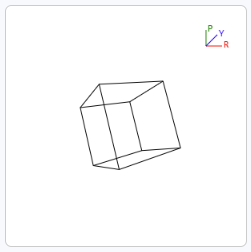
\includegraphics[width=0.4\textwidth]{img/websocket-state.PNG}
    \caption{Real-Time State Estimate Display on WebSocket}
    \label{fig:ws-state}
\end{figure}

%-------------------------------%
\paragraph{\textbf{Controller} \textit{controller.c}} \leavevmode 

Once the state estimate is and the setpoint is recieved, essentially saying \"this is my current state\" and \"this is the state I want to be in\", the realisation of the control to reach the setpoint is met through the use of a control system, in this case a cascaded \gls{pid} loop.

\temp{[PID diagram]}

\temp{Short explanation}

%-------------------------------%
\paragraph{\textbf{Stabiliser} \textit{stabiliser.c}} \leavevmode

The stabiliser ensures that all other processes in the flight controller run on time and repeatedly, acting as the centralised task from which other functions are called. A key feature is its timing system: different parts of the controller run at different frequencies using a tick-based approach. This applies both in the state estimator, which updates the attitude and position estimates, and in the controller, which computes the control outputs.  

For stabilisation, the attitude loop, controlling roll, pitch, and yaw, runs at a high frequency (500~Hz) to respond quickly to rapid angular changes. The position loop, controlling altitude and horizontal position, runs at a lower frequency (100~Hz) since translational motion is slower. This setup ensures fast dynamics are stabilised quickly, while slower dynamics are controlled efficiently.

% \begin{figure}[H]
%     \centering
%     \captionsetup{justification=centering, margin=1cm}
%     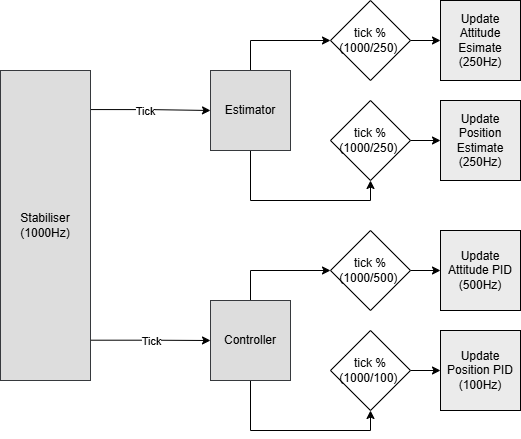
\includegraphics[width=0.65\textwidth]{img/timing.PNG}
%     \caption{Simplified Timing Decription}
%     \label{fig:arch-process}
% \end{figure}

%-------------------------------%
\paragraph{\textbf{WebSocket} \textit{websocket.c}} \leavevmode

The WebSocket interface provides a real-time connection between the flight controller and a web-based user interface. It allows the drone to send sensor readings, state estimates, and control outputs to the browser, while receiving setpoints and manual control commands from the user.  

The HTML interface displays IMU data, attitude, position, and motor outputs, and provides sliders and buttons for manual control. The WebSocket ensures that these updates are transmitted asynchronously, so the stabiliser and controller loops continue running at their required rates. Users can enable or disable motors, adjust setpoints, and request telemetry in real time, with the interface handling both periodic state updates and on-demand commands efficiently.

\temp{[Image]}

%-------------------------------%
\paragraph{\textbf{Motors} \textit{motors.c}} \leavevmode

The motors module converts the outputs of the stabiliser and controller into signals for the four drone motors. The controller outputs \textit{thrust} and attitude control corrections (\textit{roll, pitch, yaw}) which are distributed to each motor to achieve the desired motion. This is known as power distribution, and for a quadcopter in an X-configuration, the motor commands are calculated as:

\[
\begin{aligned}
M_1 &= T - \frac{R}{2} + \frac{P}{2} + Y \\
M_2 &= T - \frac{R}{2} - \frac{P}{2} - Y \\
M_3 &= T + \frac{R}{2} - \frac{P}{2} + Y \\
M_4 &= T + \frac{R}{2} + \frac{P}{2} - Y
\end{aligned}
\]

where \(M_i\) is the command for motor \(i\), \(T\) is the total thrust, \(R, P, Y\) are the roll, pitch, and yaw corrections respectively. The roll and pitch contributions are halved to balance their effect across opposing motors.  

Each motor command is then limited to a minimum \textit{idle thrust} to ensure stable spinning even when the drone is hovering:

\[
M_i = \max(M_i, T_\text{idle})
\]

Finally, these commands are converted to PWM signals for the motor ESCs, with a linear mapping from the 16-bit thrust command to the duty cycle of the PWM hardware:

\[
\text{PWM}_{i} = \text{motorConv16ToBits}(M_i)
\]

This mapping allows the controller outputs to directly control motor speeds, which in turn generate the required forces and torques to stabilise and manoeuvre the drone.

%-------------------------------------------------------------%
\subsection{Testing}

% Test No. xxx 
% Introduction for test xxx 

% Test Specification 
% Describe which requirements should be met by this test and which parts of your design are tested as well as conditions if they are different from the overall conditions/environment. 

% Test Description 
% Describe exactly how the test should be executed (input commands, data, actions, etc) and what outputs (data, signals, system messages, etc) are expected. 

% Test Result Analysis 
% Describe in which case the test is passed and what aspects of the test have to be included into a test report as deliverable. Discuss the impact of an error or test fail case. 

The testing provided a validation of the drone's hardware and firmware subsystems, serving both as proof of concept and as a diagnostic tool. Testing was conducted in two stages: \textit{Initial Stationary Testing} evaluated sensor functionality, communication protocols, and control logic without flight, while \textit{Dynamic Testing} assessed flight performance, stability, and PID control during lift-off and hovering. The Verification and Validation of for this project can be found in Appendix~\temp{V\&V To-do}.

Stationary testing confirmed that the MPU6050 IMU and VLX distance sensors functioned correctly and produced consistent readings. Integration with the Espressif EPSDrone firmware and CFClient verified reliable data acquisition and sensor interfacing. IMU calibration highlighted minor deviations in gravity measurements, which could be compensated via bias correction. The WebSocket interface was successfully implemented, enabling wireless command and telemetry communication in accordance with R.25 (User Interface). State estimation algorithms were verified visually, demonstrating accurate correspondence between estimated and actual orientation.

Concurrent development of PID control and motor command modules enabled preliminary assessment of flight dynamics. PCB integration was completed and tested to resolve hardware issues prior to flight trials. Initial motor tests on a fixed rig revealed erratic behavior, suggesting potential misalignment or calibration inconsistencies. Early hovering attempts indicated that motor instability and resource constraints limited sustained flight, emphasizing the need for further tuning of control gains and motor performance. 

Overall, the testing process validated core system functionality, identified critical limitations in motor performance and control, and provided essential data to guide subsequent design iterations and control algorithm optimization.

\subsubsection{Initial Stationary Testing} \leavevmode

Initial testing did not involve flight but focused on validating hardware and firmware components:

\begin{table}[H]
\centering
\renewcommand{\arraystretch}{1.2}
\begin{tabular}{|p{3.5cm}|p{12cm}|}
\hline
\textbf{Test No. \, \temp{XX}} & \textbf{Sensor Functionality Test} \\ \hline

\textbf{Test Specification} & 
Verify that all onboard sensors (MPU6050 IMU and VLX distance sensor) provide accurate and consistent readings. \\ \hline

\textbf{Test Description} & 
1. Power up the drone and connect via CFClient or firmware interface. \newline
2. Read accelerometer, gyroscope, and distance values while the drone remains stationary. \newline
3. Compare readings against expected physical conditions (e.g., gravity orientation for IMU, known distance for VLX). \\ \hline

\textbf{Test Result Analysis} & 
Sensors produced consistent readings within expected tolerances. Minor IMU biases were observed and could be corrected in firmware. Successful verification confirms sensors are ready for integration with control algorithms. \\ \hline
\end{tabular}
\end{table}

\begin{table}[H]
\centering
\renewcommand{\arraystretch}{1.2}
\begin{tabular}{|p{3.5cm}|p{12cm}|}
\hline
\textbf{Test No. \, \temp{XX}} & \textbf{Motor Command Verification} \\ \hline

\textbf{Test Specification} & 
Validate that motor control commands are correctly transmitted and executed without flight. \\ \hline

\textbf{Test Description} & 
1. Connect the drone to WebSocket interface. \newline
2. Send incremental motor thrust commands while drone is fixed to a test rig. \newline
3. Monitor motor responses via telemetry and visually confirm expected rotation or PWM feedback. \\ \hline

\textbf{Test Result Analysis} & 
All motor commands were received and executed appropriately. Erratic behaviour was observed only under high throttle, suggesting a need for calibration. This confirms that motor control signals are correctly delivered by the firmware. \\ \hline
\end{tabular}
\end{table}

\begin{table}[H]
\centering
\renewcommand{\arraystretch}{1.2}
\begin{tabular}{|p{3.5cm}|p{12cm}|}
\hline
\textbf{Test No. \, \temp{XX}} & \textbf{IMU Data Validation} \\ \hline

\textbf{Test Specification} & 
Confirm the accuracy of accelerometer and gyroscope data for use in state estimation and control algorithms. \\ \hline

\textbf{Test Description} & 
1. Keep the drone stationary and log accelerometer and gyroscope outputs. \newline
2. Tilt and rotate the drone slowly to produce controlled changes in orientation. \newline
3. Compare logged sensor data against expected physical motion and orientation. \\ \hline

\textbf{Test Result Analysis} & 
Sensor data corresponded closely with expected motion profiles. Small offsets were observed and noted for bias correction in the firmware. This validates that IMU measurements are reliable for state estimation and PID control integration. \\ \hline
\end{tabular}
\end{table}

\begin{table}[H]
\centering
\renewcommand{\arraystretch}{1.2}
\begin{tabular}{|p{3.5cm}|p{12cm}|}
\hline
\textbf{Test No. \, \temp{XX}} & \textbf{R.30 - Disconnection Response} (Firmware) \\ \hline

\textbf{Test Specification} & 
Ensure the drone powers off safely after loss of connection, observing motor shutdown and null setpoints. \\ \hline

\textbf{Test Description} & 
1. Connect drone to WebSocket interface. \newline
2. Send setpoints and verify terminal output. \newline
3. Close the control webpage to simulate disconnection. \newline
4. Observe if the drone detects disconnection and motors shut off. \\ \hline

\textbf{Test Result Analysis} & 
The drone successfully detected the disconnection and immediately ceased motor activity. This confirms proper handling of lost connection and application of null setpoints, meeting R.30. \\ \hline
\end{tabular}
\end{table}

%-------------------------------%
\begin{table}[H]
\centering
\renewcommand{\arraystretch}{1.2}
\begin{tabular}{|p{3.5cm}|p{12cm}|}
\hline
\textbf{Test No. \, \temp{XX}} & \textbf{R.3 - WebSocket State Estimate} (Firmware) \\ \hline

\textbf{Test Specification} & 
Validate the state estimation algorithm by comparing measured drone orientation with computed estimates. \\ \hline

\textbf{Test Description} & 
1. Tilt and manipulate drone manually while connected to WebSocket. \newline
2. Monitor state estimate output and compare with actual drone movements. \\ \hline

\textbf{Test Result Analysis} & 
The algorithm accurately tracked the drone's orientation under moderate movements. Rapid changes introduced minor lag and drift over time, indicating acceptable performance within normal operational limits. \\ \hline
\end{tabular}
\end{table}

%-------------------------------%
\subsubsection{Dynamic Testing} \leavevmode

Dynamic testing focused on lift-off, hovering, altitude maintenance, and PID stabilisation.

\begin{table}[H]
\centering
\renewcommand{\arraystretch}{1.2}
\begin{tabular}{|p{3.5cm}|p{12cm}|}
\hline
\textbf{Test No. \, \temp{XX}} & \textbf{R.2 - Capable of Hovering} (Hardware/Firmware) \\ \hline

\textbf{Test Specification} & 
Validate that the drone can lift and maintain altitude, assessing motor thrust, PID control, and manual tuning. \\ \hline

\textbf{Test Description} & 
1. Connect drone to WebSocket interface. \newline
2. Gradually increase thrust with PID disabled until lift-off occurs. \newline
3. Observe behaviour at higher thrust levels. \newline
4. Re-enable PID and attempt manual tuning of pitch/roll gains to assess stabilisation. \\ \hline

\textbf{Test Result Analysis} & 
The drone achieved lift-off; however, uneven thrust caused flipping tendencies at higher throttle. PID control did not improve stability, and manual tuning produced the same result. Likely causes include thrust misalignment or motor calibration errors rather than PID tuning. \\ \hline
\end{tabular}
\end{table}

\begin{table}[H]
\centering
\renewcommand{\arraystretch}{1.2}
\begin{tabular}{|p{3.5cm}|p{12cm}|}
\hline
\textbf{Test No. \, \temp{XX}} & \textbf{R.4 / R.2 - Hovering and Altitude Maintenance} (Hardware/Firmware) \\ \hline

\textbf{Test Specification} & 
Assess the drone's ability to achieve and maintain a stable hover at set altitude. \\ \hline

\textbf{Test Description} & 
Attempt hover with PID stabilisation active, monitoring altitude and control response via WebSocket. \\ \hline

\textbf{Test Result Analysis} & 
Hover could not be maintained due to instability. This prevented altitude evaluation and suggests issues with motor output consistency or control tuning. \\ \hline
\end{tabular}
\end{table}

\begin{table}[H]
\centering
\renewcommand{\arraystretch}{1.2}
\begin{tabular}{|p{3.5cm}|p{12cm}|}
\hline
\textbf{Test No. \, \temp{XX}} & \textbf{R.20 - Flight Stabilisation} (Hardware/Firmware) \\ \hline

\textbf{Test Specification} & 
Evaluate PID-based stabilisation and control signal application during flight. \\ \hline

\textbf{Test Description} & 
Monitor control signals and motor output during hovering attempts, observing PID response and integral windup. \\ \hline

\textbf{Test Result Analysis} & 
Hover could not be achieved, limiting assessment. Control signals were active and adjusted, but incomplete testing prevented full stabilisation. Integral windup was noted but could not be resolved. \\ \hline
\end{tabular}
\end{table}

\subsubsection{Outcome of Testing} \leavevmode

\temp{To-do}

